\chapter{Stato dell'arte}
\label{statodellarte}
All'interno di questo capitolo vengono presentate le basi teoriche che compongono il lavoro mostrato in questo elaborato. In sezione~\ref{sec:botnet} viene presentata una breve introduzione alle botnet, la loro tassonomia ed il funzionamento del Command \& Control. In Sezione~\ref{sec:machinelearning} viene introdotto il campo di studio del Machine Learning, mostrando una panoramica delle problematiche affrontabili con tale strumento ed una tassonomia delle tecniche possibili di utilizzo. In Sezione~\ref{sec:deeplearning} viene presentato il sottocampo di applicazione Machine Learning: Deep Learning, assieme ad una spiegazione dei fondamenti di funzionamento. In sezione~\ref{sec:advlearning} si espone l'argomento dell'Adversarial Learning e le problematiche che esso comporta nell'ambito dell'information security. All'interno della sezione~\ref{sec:gan} vengono mostrate le tecniche di Generative Deep Learning che saranno utilizzate all'interno di questo elaborato nei capitoli successivi quali Autoencoder e Generative Adversarial Network.

\newpage
\section{Botnet}
\label{sec:botnet}
Una botnet è composta da svariati dispositivi connessi a Internet, come host, smartphone o dispositivi IoT, ciascuno dei quali esegue uno o più bot. I proprietari delle botnet controllano queste ultime tramite software C\&C (Command and Control) per svolgere svariate attività, solitamente dannose, che richiedono un livello di automazione su vasta scala, tra cui:
\begin{itemize}
\item Attacchi DDoS (Distributed Denial-of-Service) che causano downtime non pianificati delle applicazioni
\item Verifica di elenchi di credenziali divulgate (attacchi di compilazione delle credenziali) che portano al controllo degli account
\item Attacchi alle applicazioni web allo scopo di sottrarre dati
\item Fornire a utenti malintenzionati accesso a un dispositivo e alla relativa connessione a una rete
\end{itemize}

Le botnet vengono sempre più affittate dai cyber criminali per gli scopi più diversi e rappresentano una minaccia reale per qualsiasi azienda presente in Internet. Questo significa che non è più necessario che gli autori degli attacchi siano in possesso delle conoscenze necessarie per realizzare le proprie botnet, in quanto possono utilizzare botnet già create da altri. Il numero di bot varia notevolmente da una botnet all'altra e dipende dall'abilità del proprietario della botnet di infettare dispositivi non protetti. 

Le botnet possono essere divise in due classi, operando la suddivisione per architettura (Figura~\ref{fig:botnet}):
\begin{itemize}
\item Botnet Centralizzate: il tipo di architettura è più semplice, tutti i bot sono connessi direttamente al C\&C. Il server C\&C gestisce la lista di tutte le macchine infettate, controlla il loro status e da loro informazioni operative. Questa tipologia di botnet è estremamente vulnerabile, una volta "convertito" un bot, si hanno tutte le informazioni necessarie per poter effettuare un attacco al C\&C e smantellare la rete; esistono alcune estensioni a questa struttura, in cui si usano più server di comando e controllo, ma i vantaggi che si ottengono sono trascurabili.
\item Botnet Decentralizzate o P2P: in questo schema i bot non sono necessariamente connessi al server C\&C ma tutti insieme costituiscono una rete di comunicazione in cui i comandi sono trasmessi anche da zombie a zombie. Ogni nodo della rete è un bot, il quale comunica solo con una lista di nodi “vicini”. In questo schema per gestire la botnet è necessario l'accesso ad almeno un client. Il punto di forza di questi schemi è la difficoltà che s'incontra nel momento in cui si è interessati a smantellare l'intera rete; il reverse engineering di un singolo bot non è più sufficiente a individuare tutti i computer coinvolti né tantomeno a smantellare i server C\&C.
\end{itemize}

\begin{figure}[!bp] 
  \begin{minipage}[b]{0.5\linewidth}
    \centering
    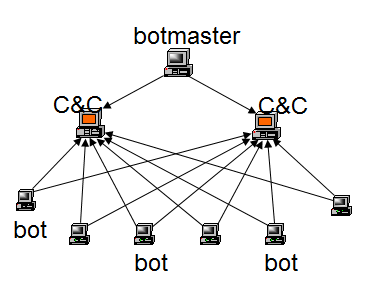
\includegraphics[width=\linewidth]{figures/botnet.png} \\ 
    Botnet Centralizzata
    \vspace{4ex}
  \end{minipage}%%
  \begin{minipage}[b]{0.5\linewidth}
    \centering
    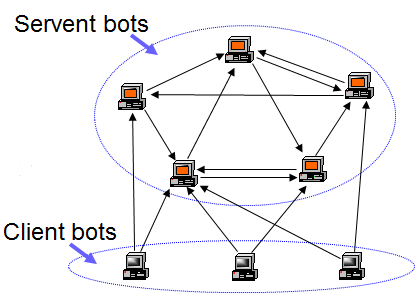
\includegraphics[width=\linewidth]{figures/botnetp2p.png} \\
    Botnet Decentralizzata 
    \vspace{4ex}
  \end{minipage} 
     \caption{Anatomia di Botnet\label{fig:botnet} }
\end{figure}

\subsection{Command and Control}
Durante la fase C\&C una macchina appena infettata diventa attivamente a far parte della botnet. Un bot tradizionale client-server, una volta installato su una nuova macchina, tenterà immediatamente il collegamento attraverso una rete IRC o contattando il server C\&C via HTTP.
I bot P2P decentralizzati ecentralised sono distribuiti con un metodo di bootstrapping predeficino per connettersi ad un DHT rilevante. Una volta connesse, le macchine compromesse chiedereanno ad uno deipropri peer riguardo gli ultimi comandi richiesti. Alcuni bot P2P richiedono che una specifica porta sia aperta ai peer per abilitare la comunicazione tra peer~\cite{p2pbots}. 
Vi sono due tecniche principali per la propagazione di comandi in un sistema botnet: push e pull.
In botnet basate su comunicazione IRC viene utilizzato il sistema push, in quanto i bot risiedono in una chat-room, in ascolto per nuovi comandi. 
In botnet basate su HTTP, i bot controllano periodicamente il server per verificare nuovi comandi. 
Reti basate su P2P possono agire in entrambe le modalità in quanto ricevono ed inviano comandi in maniera paritaria.


Molte famiglie di botnet contengono algoritmi di generazione di domini (DGA) per rendere le difese preventive inefficaci. I domini vengono generati algoritmicamente in maniera pseudo-randomica (decine di migliaia al giorno) da un campione iniziale. La macchina infetta successivamente invia una richiesta HTTP ad una larga parte di tali domini contemporaneamente, nella speranza che uno di questi domini sia effettivamente registrato e ospiti il C\&C della botnet. L'attacker ha solamente il compito di registrare un piccolo numero di questo domini, avendo a disposizione gli stessi domini generati. Dal lato dei difensori invece è necessario che tutti i domini generati da tali algoritmi siano rilevati e inseriti in una lista di esclusione per ottenere una difesa efficace della rete. Tale metodo di difesa risulta via via più inefficiente man mano che il numero di domini DGA aumenta.

\newpage
\section{Machine Learning}
\label{sec:machinelearning}
Il Machine Learning è un sottocampo dell'intelligenza artificiale (IA) è stato definito da Arthur Samuel nel 1959~\cite{5392560}. L'obiettivo del Machine Learning generalmente è capire la struttura dei dati e adattare tali dati in modelli in grado di essere capiti e utilizzati da utenti.

Nonostante il Machine Learning sia un campo informatico, si differenzia dai tradizionali approcci computazionali. Nell'informatica tradizionale, gli algoritmi sono serie di istruzioni programmate esplicitamente usate dai calcolatori per elaborare dati o risolvere problemi. Gli algoritmi Machine Learning, al contrario, permettono ai calcolatori di allenarsi su input di dati ed usare analisi statistica in modo da produrre valori che ricadono all'interno di intorni specifici. Grazie a questo, il Machine Learning facilita ai calcolatori la costruzione di modelli che siano in grado di automatizzare processi decisionali basati su campioni di dati.

Molti campi tecnologici odierni sfruttano i benefici del Machine Learning; ad esempio tecnologie di riconoscimento facciale permettono alle piattaforme di social networks di aiutare gli utenti nel tag delle foto di amici. Altro esempio sono le tecnologie di Optical Character Recognition (OCR) in grado di convertire immagini di testi stampati in documenti testuali modificabili da un word processor. I recommendation engines, basati su Machine Learning, suggeriscono agli utenti i programmi televisivi o film basati sulle loro preferenze. Le auto a guida autonoma si basano su Machine Learning in molte applicazioni, ad esempio per il riconoscimento della segnaletica stradale.

Nel Machine Learning i compiti sono generalmente classificati in grandi categorie. Tali categorie sono basate su come l'apprendimento è impostato o su come il feedback dell'apprendimento viene dato al sistema.

Due dei metodi di apprendimento più comunemente adottati sono l'apprendimento supervisionato in cui si allenano algoritmi basandosi su input e output di esempio, categorizzati da esseri umani e l'apprendimento non supervisionato, in cui non vengono forniti dati categorizzati agli algoritmi in modo da permettere al sistema di trovare autonomamente la struttura che compone i dati di input. Nelle sezioni seguenti si mostrano tali metodi in dettaglio.

\subsection{Tipologie di Problemi}
Il Machine Learning è impiegato principalmente per la risoluzione di tre tipologie di problemi:

\begin{itemize}
\item \textbf{classificazione}, ovvero identificare la classe di un nuovo obiettivo sulla base di conoscenza estratta da un training set. I classificatori estraggono dal dataset un modello che utilizzano poi per classificare le nuove istanze. Se una singola istanza può essere espressa come un vettore in uno spazio numerico $R^n$ il problema della classificazione può essere ricondotto alla ricerca delle superfici chiuse che delimitano le classi. Esistono molte tecniche per costruire un classificatore, in questa tesi si tratterà in particolare l'uso di Alberi di Decisione. Si tratta di un classificatore implementato attraverso una struttura ad albero; è quindi costituito da una struttura gerarchica che applica una strategia “dividi et impera” per classificare i dati. Data la sua struttura di albero può essere facilmente convertito in un set di regole, permettendo così di estrarre conoscenza. La ricerca delle curve che delimitano le classi viene ricondotta alla ricerca ricorsiva di punti di split.
Ogni nodo interno rappresenta un vincolo che porta a una scelta determinando uno split, e ogni foglia indica la classe di appartenenza dell’elemento. Gli alberi sono tipicamente costruiti con strategie Greedy, che individuano di volta in volta il punto più conveniente in cui effettuare lo split. (Figura~\ref{fig:alberoastratto}).

\begin{figure}[!h]
	\centering
	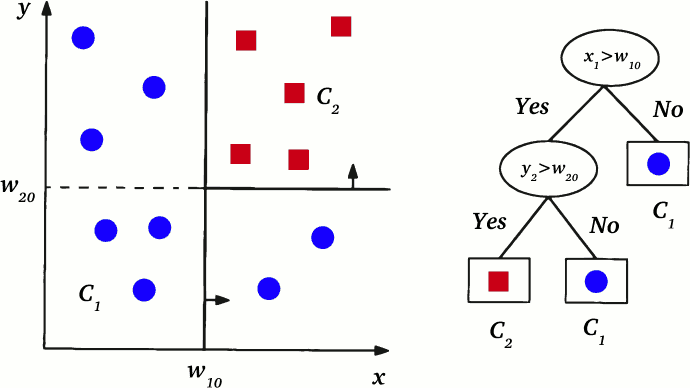
\includegraphics[width=\columnwidth]{figures/AlberoAstratto.png}
	\caption{Utilizzo di un albero per la classificazione di un dataset \label{fig:alberoastratto}}
\end{figure} 

\item \textbf{raggruppamento} (clustering), quando si vuole raggruppare i dati che presentano caratteristiche simili. Ad esempio, un sistema può raggruppare immagini di figure geometriche separando figure con 4 lati e i cui angoli sono a 90 gradi oppure tutte le figure con quattro lati in cui solo due sono paralleli, ecc. In marketing, ad esempio, il raggruppamento viene utilizzato per l'individuazione di clienti e mercati potenziali.
\item \textbf{regressione}, cioè prevedere il valore futuro di un dato avendo noto il suo valore attuale. Un esempio è la previsione della quotazione delle valute o delle azioni di una società. Nel marketing viene utilizzato per prevedere il tasso di risposta di una campagna sulla base di un dato profilo di clienti; nell'ambito commerciale per stimare come varia il fatturato dell'azienda al mutare della strategia.
\end{itemize}

\subsection{Apprendimento Supervisionato}
Nell'apprendimento supervisionato, vengono forniti al sistema dei dati di input già etichettati con l'output desiderato. Lo scopo di tale metodo è permettere all'algoritmo di apprendimento di imparare comparando il suo output con quello fornito in ingresso, in modo da rilevare errori e modificare il modello di conseguenza. L'apprendimento supervisionato perciò usa patterns per predire i valori delle "etichette" su dati non etichettati.

Ad esempio, con l'apprendimento supervisionato, si può fornire ad un algoritmo un insieme di immagini di squali, etichettati come $pesce$ e immagini di oceani etichettati come $acqua$. Allenandosi su tali dati, l'algoritmo supervisionato dovrebbe essere in grado di riconoscere immagini di squali ed etichettarle come $pesci"$ ed immagini di oceani ed etichettarle come $acqua$.

Un comune uso dell'apprendimento supervisionato è l'uso di dati storici per predire probabili eventi futuri. Può usare informazioni statistiche sull'andamento del mercato azionario ed anticipare fluttuazioni future o utilizzato per filtrare email di spam. E' possibile utilizzare foto di cani etichettate per identificare la razza di un cane unicamente dalla sua foto.

\subsection{Apprendimento non Supervisionato}
Nell'apprendimento non supervisionato, i dati non sono etichettati. L'algoritmo viene lasciato libero di rilevare affinità tra i dati di input. Siccome i dati non classificati sono molto piu comuni che grandi quantità di dati etichettati, i metodi di Machine Learning che facilitano l'apprendimento non supervisionato sono considerabili come molto pregiati.

L'obiettivo dell'apprendimento non supervisionato può essere diretto, come la ricerca di pattern nascosti all'interno dei dati, ma può anche avere l'obiettivo di \textit{feature learning}: l'apprendimento di caratteristiche particolari che permette al sistema di scoprire automaticamente le rappresentazioni necessarie a classificare i dati grezzi.

L'apprendimento non supervisionato viene comunemente utilizzato per dati transazionali. Ad esempio, nel caso reale di un grosso dataset di clienti e dei loro acquisti, un essere umano difficilmente riuscirebbe a ricavare gli attributi che legano i profili clienti e le tipologie dei loro acquisti. Tuttavia fornendo tali dati ad un algoritmo di  apprendimento non supervisionato è possibile rilevare caratteristiche che legano determinati gruppi di clientela a determinati prodotti e di conseguenza prendere decisioni di marketing mirate.

L'apprendimento non supervisionato, grazie alla mancanza di un target da raggiungere, è in grado di analizzare dati che   apparentemente non mostrano relazioni ed estrarne dati significativi. Viene spesso usato per eseguire \textit{anomaly detection}, come l'utilizzo fraudolento di carte di credito; oppure è possibile eseguire classificazione di immagini (come nel precedente caso di razze canine) in maniera autonoma partendo da immagini non categorizzate.

\subsection{Apprendimento Semi Supervisionato}
Posto a metà tra il supervisonato e il non-supervisionato, l'apprendimento parzialmente supervisionato si basa su dati misti in cui una minima parte è già etichettata e una larghissima maggioranza è costituita da dati non etichettati.  Questo approccio viene utilizzato per migliorare le previsioni fatte dalla macchina sui dati non etichettati e richiede, normalmente, l'intervento di un analista. L'approccio è principalmente usato nei problemi di classificazione e di raggruppamento o nella descrizione delle relazioni causa-effetto tra le variabili.

\subsection{Apprendimento per Rinforzo}
L'apprendimento per rinforzo (Reinforcement learning) è una tecnica di apprendimento automatico che punta a realizzare sistemi in grado di apprendere ed adattarsi ai cambiamenti dell'ambiente in cui sono immersi attraverso la distribuzione di una “ricompensa” detta rinforzo, data dalla valutazione delle prestazioni.
Il suo funzionamento è attuato da tre componenti:
\begin{itemize}
\item un sistema logico di esecuzione (definito A), che sulla base dei dati in ingresso (Input) riesce a restituire un risultato (Output)
\item un sistema logico di valutazione (definito B) che assegna un premio (se il risultato è corretto) o una penalità (se il risultato non è corretto) al sistema logico A
\item un sistema logico di ottimizzazione (definito C) che osserva il comportamento di A e B e modifica il modello utilizzato da A per aumentare il premio e ridurre le penalità che B assegna ad A.
\end{itemize}

L'apprendimento per rinforzo è utilizzato in tutti quei campi in cui è essenziale che la macchina risponda ai cambiamenti dell'ambiente. Per questo è utilizzato frequentemente nella robotica, per controllare i movimenti degli automi, ma anche nelle auto a guida autonoma. Trova anche applicazione in ambiti industriali nella produzione e nel controllo qualità e in diversi altri settori.



\newpage
\section{Deep Learning e Reti neurali}
\label{sec:deeplearning}
Il Deep Learning è uno specifico sottocampo del Machine Learning, un diverso modo di apprendere rappresentazioni di dati, principalmente orientato verso l'apprendimento di successivi strati (\textit{layers}) di rappresentazione via via più significativi. Il termine "deep" indica la presenza di questa moltitudine di strati che compongono il modello
di rappresentazione dei dati; infatti il deep learning odierno comprende generalmente modelli composti da decine o centinaia di strati successivi di rappresentazione, i quali apprendono in maniera automatica tramite l'esposizione ai dati di allenamento. Per confronto, gli approcci di Machine Learning descritti in sezione~\ref{sec:machinelearning} generalmente coinvolgono uno o due strati di rappresentazione dei dati. Difatti tali modelli vengono definiti anche come \textit{shallow learning}.
 
\begin{figure}[!bp]
	\centering
	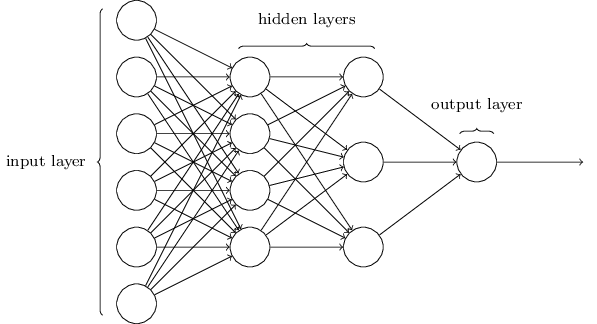
\includegraphics[width=\columnwidth]{figures/mlp-network.png}
	\caption{Schema generico di una rete Neurale \label{nn}}
\end{figure} 
 
All'interno del deep learning, queste rappresentazioni a più strati sono quasi unicamente apprese attraverso modelli definiti \textbf{reti neurali}, strutturati letteralmente in strati sovrapposti gli uni agli altri. Il termine "rete neurale" deriva dal campo della neurobiologia, tuttavia non si tratta di veri e propri modelli del funzionamento del cervello umano.

\begin{figure}[!bp]
	\centering
	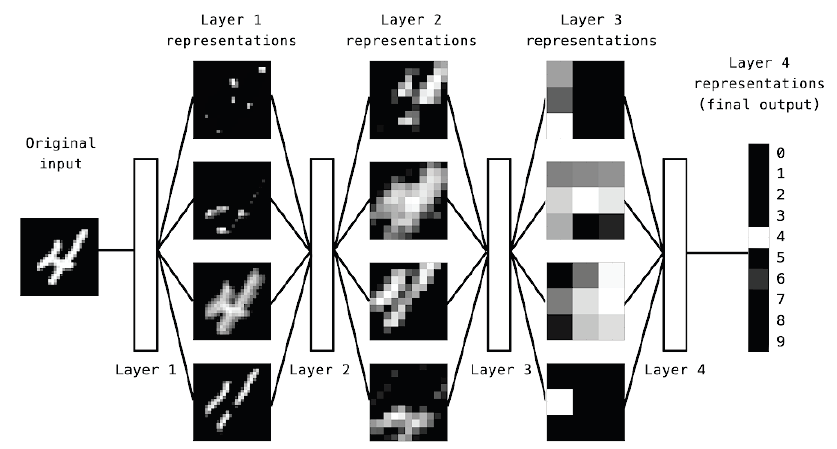
\includegraphics[width=\columnwidth]{figures/deeplearning.png}
	\caption{Esempio di rappresentazione di una cifra numerica tramite rete neurale. \textit{fonte}%
	~\cite{chollet2017deep} \label{fig:neuralnetwork} }
\end{figure}

Come è possibile vedere in figura~\ref{fig:neuralnetwork}, la rete neurale trasforma l'immagine di una cifra numerica disegnata a mano in una rappresentazione via via più informativa riguardo il risultato finale. Si può considerare il deep leraning come una operazione di distillazione di informazioni composta da più fasi in cui i dati vengono filtrati in maniera sempre più fine.

\subsection{Funzionamento Reti Neurali}
Le informazioni specifiche riguardo quali operazioni un livello apporta ai dati di input sono immagazzinate all'interno degli strati stessi, nella matrice dei "pesi". La trasformazione implementata da un livello è parametrizzata da tali pesi. Generalmente la fase di apprendimento consiste nel trovare un set di valori per i quali i pesi di tutti gli strati che compongono una rete neurale mappino correttamente i dati di esempio ai loro target associati.
Tuttavia l'operazione di ricerca dei valori ottimali non è triviale, in quanto una rete neurale può contenere fino a decine di milioni di parametri e rilevarne i valori corretti risulta in una operazione complessa.

Per superare tale vincolo, la fase di apprendimento di una rete neurale è composta da più fasi di osservazione, nel quale si misura quanto distante si trova l'output da quanto atteso. Tale è il compito della funzione di \textit{loss}. La funzione di loss utilizza la predizione della rete neurale e l'output atteso e computa un punteggio di distanza, catturando quindi la performance della rete sull'esempio analizzato.

Il meccanismo principale nel deep learning è l'uso di questo punteggio come segnale di \textit{feedback} per aggiustare il valore dei pesi in maniera da diminuire il valore del punteggio di loss per l'esempio analizzato. Questo aggiustamento è compito dell'\textit{ottimizzatore}, il quale implementa l'algoritmo di \textit{backpropagation} che attua la modifica dei pesi durante la fase di apprendimento.

Inizialmente i pesi della rete neurale sono assegnati a valori randomici, causando per le prime fasi di apprendimento un valore di loss particolarmente alto. Via via che le fasi di apprendimento mostrano diversi esempi alla rete i pesi vengono aggiustati di una piccola parte nella direzione corretta, causando una decrescita nel punteggo di loss. Questo \textit{training loop} viene ripetuto per un numero sufficiente di volte fino al raggiungimento di un valore minimo di loss e alla produzione di output il più possibile simile a quello desiderato. In figura~\ref{fig:neuralloss} è mostrato uno schema di alto livello.

\begin{figure}[!bp]
	\centering
	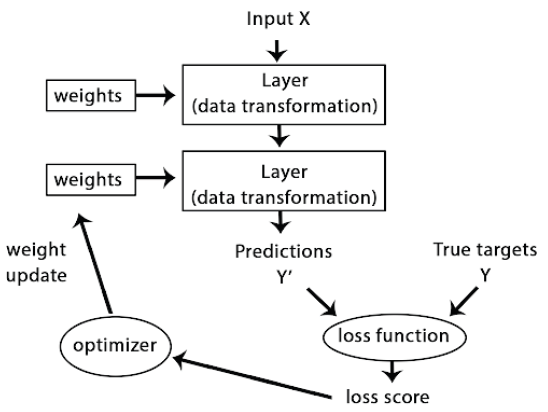
\includegraphics[width=0.8\columnwidth]{figures/deeploss.png}
	\caption{Schema di alto livello del funzionamento di una rete neurale. \textit{fonte}%
	~\cite{chollet2017deep} \label{fig:neuralloss} }
\end{figure}

\newpage
\section{Adversarial Learning}
\label{sec:advlearning}
Le tecniche di Machine Learning possono essere utilizzate per prevenire azioni vietate o illegali e nel caso vi siano degli incentivi economici, vi possono essere probabili antagonisti intenzionati ad eludere tali restrizioni. Un esempio tipico è il caso del filtraggio anti spam, nel quale gli spammers forgiano messaggi ad hoc per eludere le più recenti tecniche di filtraggio. Tali tecniche possono essere identificate come \textit{adversarial learning} (apprendimento antagonista).

Le vulnerabilità dei metodi di Machine Learning rispetto a manipolazione antagonista non possono venire semplicemente ignorate con la richiesta di tecniche più "robuste". I fondamenti teorici del Machine Learning odierno sono largamente costruiti sull'assunto che i dati di allenamento descrivano adeguatamente la realtà del fenomeno studiato. Questo assunto viene chiaramente violato nel caso che le distribuzioni di allenamento o di test vengano alterate, assumendo che gli antagonisti utilizzino qualsiasi mezzo possibile per disturbare l'algoritmo di apprendimento. I metodi di apprendimento in caso di ambienti antagonisti dovrebbero quindi essere in grado di sostenere una distorsione nei propri dati.

Come dimostrato da ricerche precedenti (~\cite{kearnsli},~\cite{Auer2002},~\cite{paclearning} ) un antagonista senza vincoli che può arbitrariamente alterare dati e target, può introdurre un errore fino al 100\%. Tuttavia nei casi pratici gli attackers devono atteneresi a determinati vincoli; ad esempio una email di spam deve recapitare il suo messaggio, un malware inviato ad un host deve eseguire correttamente e sfruttare una vulnerabilità e antagonisti che cercano di alterare i motori di ricerca possono controllare solo una frazione di tutti i domini raggiungibili. In alcuni casi si può mostrare come certi vincoli possono rendere la rilevazione di un attacco computazionalmente intrattabile~\cite{fogla}.

L'investigazione di metodi di Machine Learning per ambienti ostili è stata attuata in tre aree di ricerca largamente distinte: Machine Learning, sicurezza informatica e spam filtering. Nel caso di Machine Learning ricerche precedenti si sono incentrate su metodi di minimo-massimo con l'obiettivo di ottenere robustezza rispetto alla incertezza dell'input. Ad esempio classificatori più robusti sono stati sviluppati per gestire casi come il feature deletion~\cite{globerson} ; oppure ricerche hanno dimostrato che equilibri unici di Nash esistono per alcune tipologie di situazioni antagoniste~\cite{nash} .

Una differente visione dei problemi di apprendimento antagonista è emersa nel campo della sicurezza informatica, specialmente per quel che riguarda il rilevamento di intrusioni (\textit{intrusion detection} ). Diversi metodi sono stati proposti per rilevare pacchetti di rete anomali o per generare automaticamente \textit{signatures} strettamente legate a metodi di Machine Learning (ad esempio i lavori eseguiti in~\cite{wangstolfo} e~\cite{wang2006} ).

L'area dello spam filtering ha richiesto sforzi fondamentali da parte degli esperti in sicurezza; la costante ricerca di tecniche di evasione dei filtri anti-spam ha portato a studi estensivi riguardo vincoli e tecniche robuste di filtering~\cite{dalvi}. 

Il Machine Learning può fornire soluzione a difficili problemi di sicurezza di rete, compresi filtri anti-spam, rilevazione di vari tipologie di attacchi contro server e host, rilevazione di pagine web deliberatamente modificate per manipolare i motori di ricerca sfruttandone le vulnerabilità. Tutte queste problematiche riguardano la manipolazione di grandi quantità di dati in un ambiente altamente variabile e il bisogno di tecniche di classificazione veloci ed accurate. L'esistenza di antagonisti che possono trarre profitto in queste aree complica l'applicazione di Machine Learning e crea una "corsa agli armamenti" tra chi sviluppa classificatori sempre piu robusti e antagonisti che cercano di manipolare tali classificatori. Fortunatamente ogni area di applicazione fornisce vincoli riguardo le azioni antagoniste che rendono la classificazione fattibile. 

\begin{figure}[!bp]
	\centering
	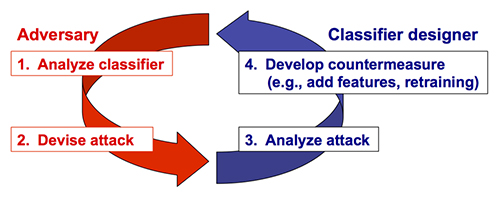
\includegraphics[width=\columnwidth]{figures/Reactive_arms_race.jpg}
	\caption{Schema concettuale del rapporto tra difensori ed antagonisti. \textit{fonte}%
	~\cite{wiki:Adversarial_machine_learning} \label{fig:advarms} }
\end{figure}


\newpage
\section{Generative Deep Learning}
\label{sec:gan}
I recenti risultati ottenuti nell'ambito del Machine Learning e del deep learning hanno permesso di ottenere algoritmi e architetture in grado di modellare complesse strutture di dati come immagini, suoni e testo. Questi avanzamenti sono stati incentrati principalmente in algoritmi di apprendimento supervisionato in grado di stimare una distribuzione di probabilità $p(x|y)$ dato un input ed un output di target. Tali modelli vengono definiti come modelli discriminativi o predditivi.

I modelli Generativi, al contrario, tentano di apprendere una funzione $p(y,x)$ nota come \textit{probabilità congiunta}. Tali funzioni di probabilità sono correlate secondo la relazione: 
\[p(x,y)=p(x)p(x|y)\]
dove $p(x)$ indica la densità di probabilità per l'evento $x$. 
Nel caso di modelli generativi, il modello ha accesso alla probabilità di input ed output allo stesso istante; permettendo ad esempio di generare immagini di animali, campionando specie di animali $y$ e nuove immagini $x$ a partire da $p(x,y)$.
Il passo successivo è l'abilità di apprendere solo la funzione di densità $p(x)$, dipendente unicamente dallo spazio degli input. Tali algoritmi sono definiti come Modelli Generativi non Supervisionati (\textit{Unsupervised Generative Models}), dove il termine \textit{generativo} indica l'abilità di campionare dalla distribuzione catturata dal modello. 

L'idea fondamentale alla base dei modelli generativi è la volontà di convertire il problema di generazione di dati in un problema di predizione ed usare l'insieme di tecniche di deep learning già note per risolvere tale problema. Gli algoritmi di deep learning odierni sono in grado di modellare mappature molto complesse e offrono flessibilità nel definire problemi in termini di grafi computazionali che possono essere ottimizzati da varianti di algoritmi di back-propagation.

\subsection{Autoencoder}
La forma più semplificata di conversione da problema generativo a problema discriminativo è l'apprendimento di una mappatura a partire dallo spazio degli input stesso. Sia dato un input $x$, si vuole ottenere una identità di tale input $x=f(x)$ dove $f$ rappresenta il modello predittivo. Il modello generativo può essere definito come l'insieme formato da un modello \textit{encoder} $q_e(h|x)$ in grado di mappare l'input in un nuovo spazio, definito come \textit{spazio latente} rappresentato da $h$ ed un modello \textit{decoder} $q_d(x|h)$ in grado di apprendere la mappatura inversa a partire dallo spazio latente.
Queste due componenti possono essere connesse assieme, a formare un modello end-to-end allenabile, caratterizzato da un vincolo di dimensione nello spazio latente $h$; generalmente definito come una riduzione di dimensione con lo scopo di far apprendere al modello un vettore di caratteristiche fondamentali dell'input. (figura~\ref{fig:aut}

\begin{figure}[!bp]
	\centering
	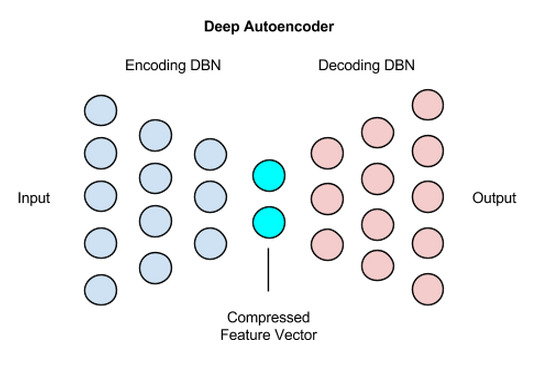
\includegraphics[width=\columnwidth]{figures/deep_autoencoder.png}
	\caption{Schema concettuale di un Autoencoder.  \label{fig:aut} }
\end{figure}

Una volta che il modello è stato appreso, decoder ed encoder possono essere utilizzati indipendentemente, ad esempio per generare nuovi campioni a partire dallo spazio latente.

\subsection{Generative Adversarial Networks}
La naturale evoluzione delle architetture Autoencoder è la Generative Adversarial Network in cui encoder e decoder vengono rimodellati due reti :discriminatore e generatore. 

Con l'obiettivo di apprendere la distribuzione del \textit{generatore} $p_g$ rispetto ai dati $\bm{x}$, si definisce precedentemente una variabile di rumore input  $p_{\b{z}}(\bm{z})$, e successivamente si rappresenta una mappatura dello spazio dei dati come $G(\bm{z}; \theta_g)$, dove $G$ è una funzione differenziabile rappresentata da una rete neurale a parametri $\theta_g$. Si definisce inoltre una seconda rete neurale \textit{discriminatore}
 $D(\bm{x}; \theta_d)$ che emette un singolo scalare. $D(\bm{x})$ rappresenta la probabilità che tale $\bm{x}$ provenga dai dati reali piuttosto che da $p_g$. 
A tal scopo si allena $D$ per massimizzare la probabilità di assegnare l'etichetta corretta sia ai campioni di allenamento che a quelli provenienti da $G$.
Simultaneamente si allema $G$ per minimizzare $\log(1-D(G(\bm{z})))$:

In altri termini, $D$ e $G$ eseguono una partita a due giocatori di minimo-massimo con funzione di valore $V(G, D)$: 

\begin{equation}
\label{eq:minimaxgame-definition}
\min_G \max_D V(D, G) = \mathbb{E}_{\bm{x} \sim p_{\text{data}}(\bm{x})}[\log D(\bm{x})] + \mathbb{E}_{\bm{z} \sim p_{\bm{z}}(\bm{z})}[\log (1 - D(G(\bm{z})))].
\end{equation}

In pratica è necessario implementare la partita in maniera iterativa. L'ottimizzazione di $D$ fino al completamento in un training a se stante risulta computazionalmente proibitivo e su dataset finiti risulta nel fenomeno di \textit{overfitting}. In maniera differente si alternano $k$ passi di ottimizzazione di $D$ ed un passo di ottimizzazione di $G$. Questo risulta nel mantenimento di $D$ vicino alla sua soluzione ottimale, cambiando gradualmente $G$. Questa strategia è mostrata formalmente all'interno dell'algoritmo~~\ref{alg:AGF}.

In pratica l'equazione~~\ref{eq:minimaxgame-definition} può non fornire un gradiente sufficiente per permettere a $G$ di apprendere. Nelle fasi iniziali dove $G$ è debole, $D$ può rifiutare i campioni con buona certezza in quanto chiaramente differenti dai dati di training. In tal caso, $\log ( 1- D(G(\bm{z})))$ satura. Piuttosto che allenare $G$ al fine di minimizzare $\log (1 - D(G(\bm{z})))$ si allena per massimizzare $\log D(G(\bm{z}))$. 
Questa funzione obiettivo risulta nello stesso punto fisso che forma la dinamica di $G$ and $D$ ma fornisce un gradiente molto più stabile nelle fasi iniziali.

In figura~\ref{fig:intuition} viene mostrata la fase di apprendimento di una GAN. Tale architettura è allenata aggiornando simultaneamente il gradiente della distribuzione discriminativa ($D$, linea blu tratteggiata) in modo che discrimini tra campioni della distribuzione generatrice di dati (linea nera tratteggata) $p_{\bm{x}}$ e i campioni provenienti dalla distribuzione del generatore $p_g$ (G) (linea verde).
La linea nera orizzontale da cui $\bm{z}$ è campionato è in questo caso uniforme; mentre la linea nera superiore è parte del dominio di $\bm{x}$. Le frecce indicano come la mappatura $\bm{x}=G(\bm{z})$ imponga una distribuzione non uniforme $p_g$ sui campioni trasformati. $G$ si contrae in regioni ad alta densità ed espande in regioni a bassa densità $p_g$. 
Di seguito la descrizione di quanto mostrato in figura~\ref{fig:intuition}
\begin{itemize}
\item (a) si considera una coppia avversaria prossima alla convergenza: $p_g$ è simile a $p_\text{data}$ e
$D$ è un classificatore parzialmente accurato.

\item (b) Nell'iterazione interna dell'algoritmo, $D$ è allenato a discriminare dati convergenti da:

\[D^*(\bm{x}) = 
\frac{
    p_\text{data}(\bm{x})
    }{
        p_\text{data}(\bm{x}) + p_g(\bm{x})}
\]

\item (c) dopo un aggiornamento a $G$, il gradiente di $D$ ha guidato $G(\bm{z})$ verso regioni dove sia più probabile che sia classificato come dato.

\item (d) dopo numerosi step di training se $G$ e $D$ hanno sufficiente capacità, raggiungono entrambi un punto in cui entrambi non possono migliorarsi a causa di \[p_g = p_\text{data}\] Il discriminatore non è in grado di differenziare tra le due distribuzioni. (ad esempio: $D(\bm{x}) = \frac{1}{2}$).
\end{itemize}

\begin{figure}[p] 
  \begin{minipage}[b]{0.5\linewidth}
    \centering
    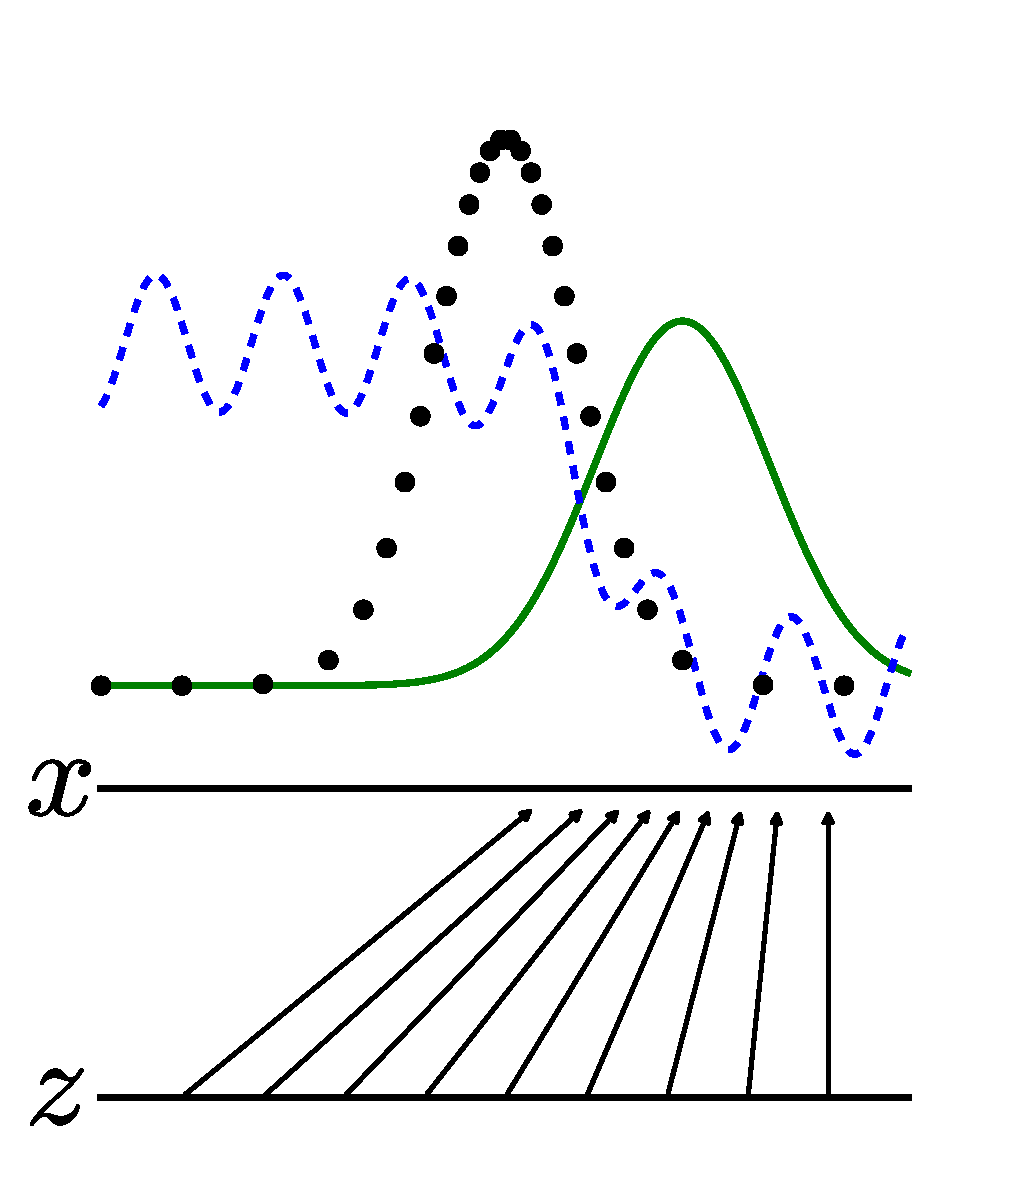
\includegraphics[width=.9\linewidth]{figures/fig1.pdf} \\ 
    (a)
    \vspace{4ex}
  \end{minipage}%%
  \begin{minipage}[b]{0.5\linewidth}
    \centering
    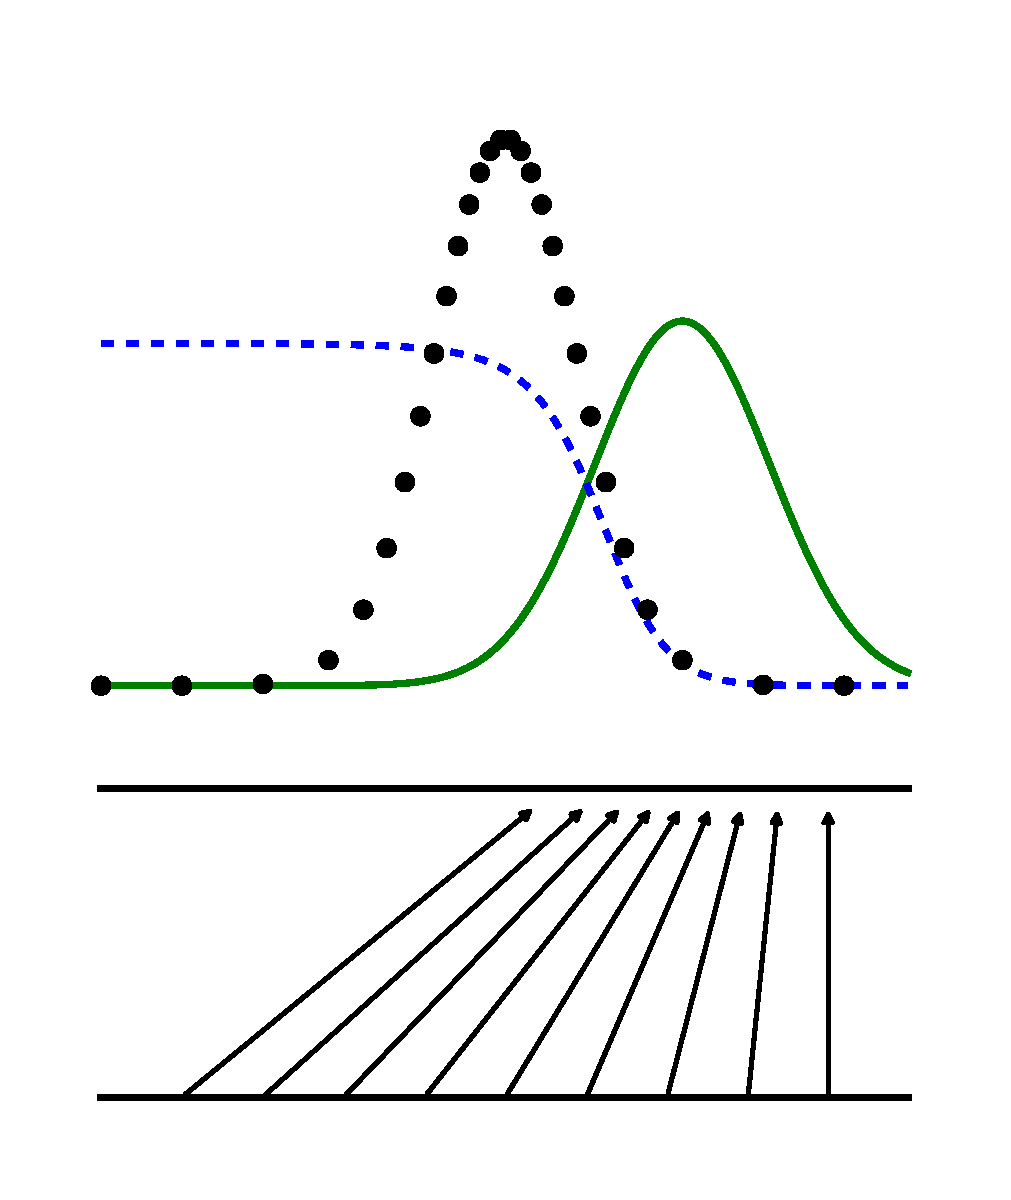
\includegraphics[width=.9\linewidth]{figures/fig2.pdf} \\
    (b) 
    \vspace{4ex}
  \end{minipage} 
  \begin{minipage}[b]{0.5\linewidth}
    \centering
    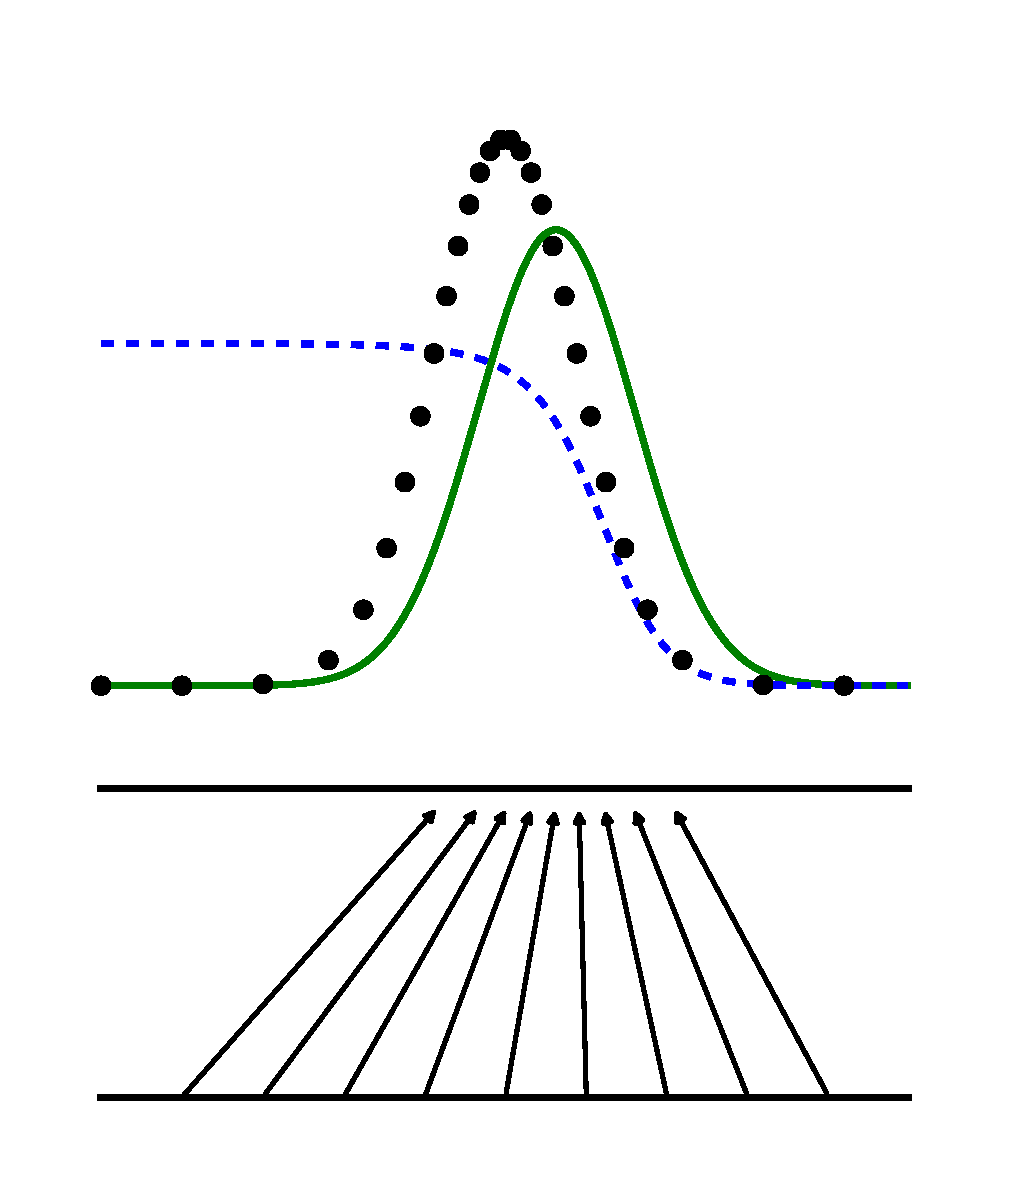
\includegraphics[width=.9\linewidth]{figures/fig3.pdf}  \\
    (c) 
    \vspace{4ex}
  \end{minipage}%% 
  \begin{minipage}[b]{0.5\linewidth}
    \centering
    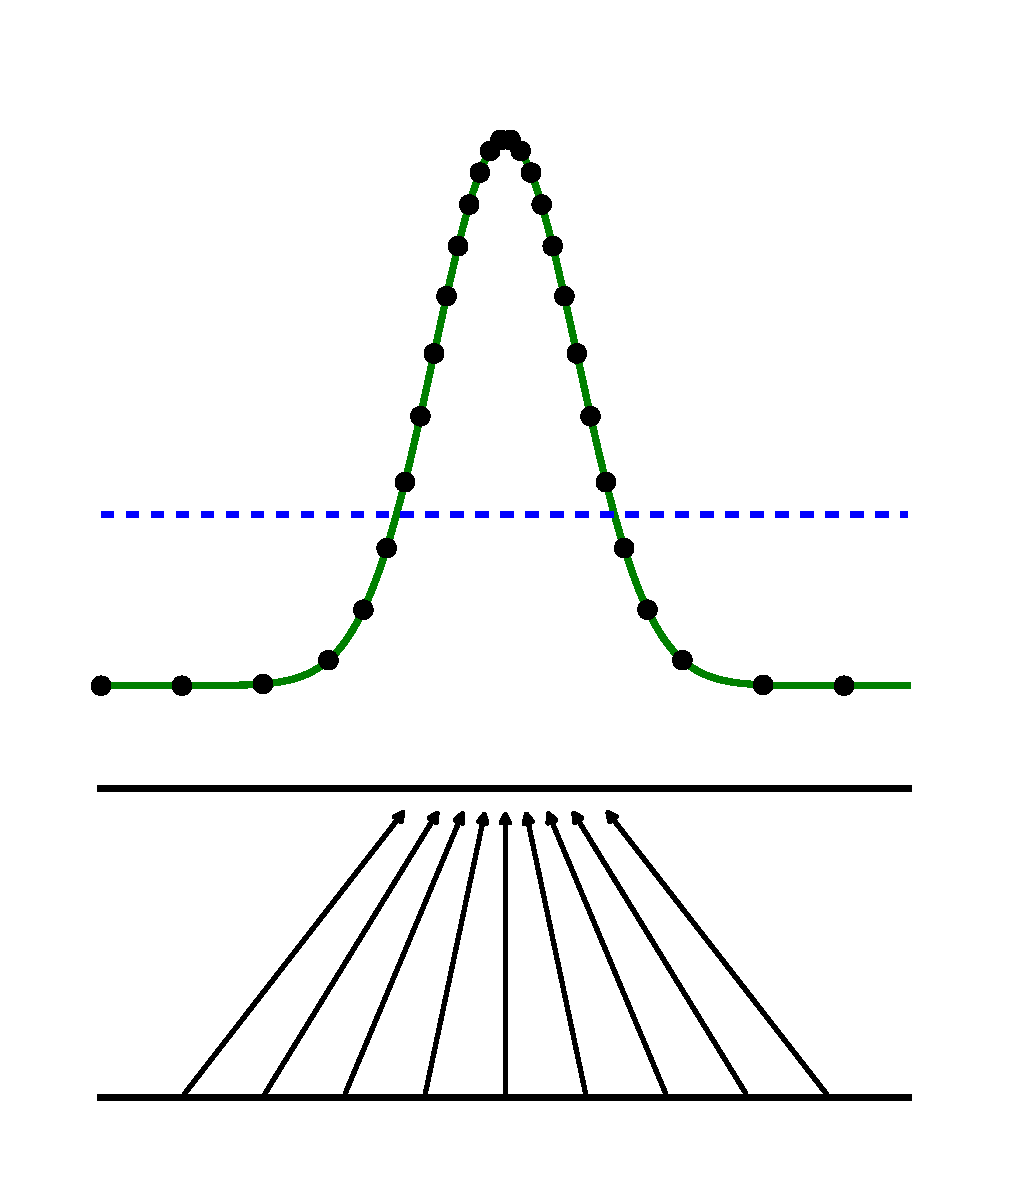
\includegraphics[width=.9\linewidth]{figures/fig4.pdf} \\
   (d) 
    \vspace{4ex}
  \end{minipage}
   \caption{\label{fig:intuition} }
 
\end{figure}

Il minimo globale del criterio di training virtuale $C(G)$ è ottenuto solo se $p_g=p_\text{data}$. 
A tal punto, si raggiungerà il valore $C(G) = -\log 4$. 
Se $G$ e $D$ hanno sufficiente capacità e ad ogni step dell'algoritmo~\ref{alg:AGF} il discriminatore è in grado di raggiungere il suo ottimo dato $G$, ed inoltre se $p_g$ venga aggiornato così da migliorare il criterio 
\[\mathbb{E}_{\bm{x} \sim p_\text{data}}[\log D^*_G(\bm{x})] + \mathbb{E}_{\bm{x} \sim p_g}[\log (1 - D^*_G(\bm{x}))]\] 
allora $p_g$ convergerà a $p_\text{data}$.

\subsubsection{Vantaggi e Svantaggi}
Questo framework moderno presenta vantaggie  e svantaggi relativi ai precedenti framework. Gli svantaggi primariamente sono che non esiste una esplicita rappresentazione di $p_g(\bm{x})$, e che $D$ deve essere ben sincronizzato con $G$ durante la fase di training (in particolare, $G$ non deve essere allenato troppo senza aggiornare $D$, in modo da evitare uno scenario degenerativo in cui $G$ collassa troppi valori di $\mathbf{z}$ verso lo stesso valore di $\mathbf{x}$ per ottenere abbastanza diversità da modellare $p_\text{data}$). 
I vantaggi rispetto a modelli alternativi come le Catene di Markov sono principalmente di tipo computazionale. I modelli antagonisti possono trarre un vantaggio statistico non dovendo aggiornare la rete generatrice con campioni di dati ma solamente tramite il flusso di gradiente che attraversa il discriminatore. Questo significa che le componenti dell'input non sono copiate direttamente nei parametri del generatore. Un ulteriore vantaggio delle reti antagoniste è la capacità di rappresentare distribuzioni molto nette mentre metodi alternativi basati su Catene di Markov richiedono che la distribuzione sia meno distinta in modo da garantire alle catene la capacità di mischiare le modalità.

\begin{algorithm}[p]
\caption{Discesa stocastica del gradiente durante la fase di training di una GAN.
il numero di passi applicati al discriminatore, $k$, è un iperparametro della rete.
}
\begin{algorithmic}
\label{alg:AGF}
\FOR{numero di iterazioni di trainingons}
  \FOR{$k$ passi}
    \STATE{$\bullet$ Campionare un mini-batch di $m$ campioni generati da rumore $\{ \bm{z}^{(1)}, \dots, \bm{z}^{(m)} \}$ dal rumore precedente $p_g(\bm{z})$.}
    \STATE{$\bullet$ Campionare un mini-batch di $m$ esempi $\{ \bm{x}^{(1)}, \dots, \bm{x}^{(m)} \}$ dalla distribuzione di dati reali $p_\text{data}(\bm{x})$.}
    \STATE{$\bullet$ Aggiornare il discriminatore aumentando il proprio gradiente stocastico:
        \[
            \nabla_{\theta_d} \frac{1}{m} \sum_{i=1}^m \left[
            \log D\left(\bm{x}^{(i)}\right)
            + \log \left(1-D\left(G\left(\bm{z}^{(i)}\right)\right)\right)
            \right].
        \]}
    %parameters $\theta_d$ of discriminator $D$
   %in the direction of the stochastic gradient of the binomial cross-entropy
   %for $D$ predicting whether its argument comes from $p_\text{data}(\bm{x})$ (target = 1, input = $\bm{x}$) or
   %$P_g$ (target = 0, input = $G(\bm{z})$), i.e., towards minimizing
   % \mbox{$-\log D(\bm{x}) - \log(1 - D(G(\bm{z})))$}.}
   \ENDFOR
  \STATE{$\bullet$ Campionare un mini-batch di $m$ campioni generati da rumore $\{ \bm{z}^{(1)}, \dots, \bm{z}^{(m)} \}$ dal rumore precedente $p_g(\bm{z})$.}
    \STATE{$\bullet$ Aggiornare il generatore, aumentando il proprio gradiente stocastico:
        \[
            \nabla_{\theta_g} \frac{1}{m} \sum_{i=1}^m
            \log \left(1-D\left(G\left(\bm{z}^{(i)}\right)\right)\right)
            .
        \]}
  \ENDFOR
  \\Gli aggiornamenti di gradiente possono utilizzare qualsiasi legge di apprendimento.
  \end{algorithmic}
\end{algorithm}



